As explained in the above section, getblocktemplate was coded into Bitcoin Core as any other RPCs, so it was (and it still is) perfectly usable by anyone who has got a Bitcoin full node. However, the main reasons which took to its development, derived from the ever-growing context of pooled mining. \\
Because of this, the focus will be about how GBT works and how it was used as a communication mining protocol between single miners and mining pools.\\\\
First, the miner must connect to the pool server, asking for an initial block template. There can be only one JSON Object in the request, containing request parameters (divided in "capabilities" and "mode"):
\begin{verbatim}
{
    "id": 0, 
    "method": "getblocktemplate", 
    "params": 
    [{
      "mode": "template", (or "proposal")	
      "capabilities": ["coinbasetxn", "workid", "coinbase/append"],
    }]
}
\end{verbatim}

\begin{figure}[h!]
\centering
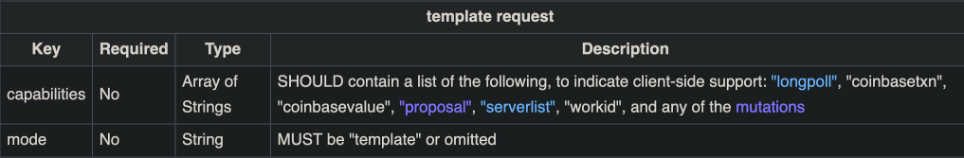
\includegraphics[width=15cm]{Figures/gbt/gbt2.png}
\caption{Description of the initial block template request parameters, using GBT}
\label{fig:gbt2}
\end{figure}

\noindent In the template request, the miner can indicate to pool server the features supported client-side, such as "longpoll", specifying the desired mutations in the "capabilities" field. \newpage

\begin{figure}[h!]
\centering
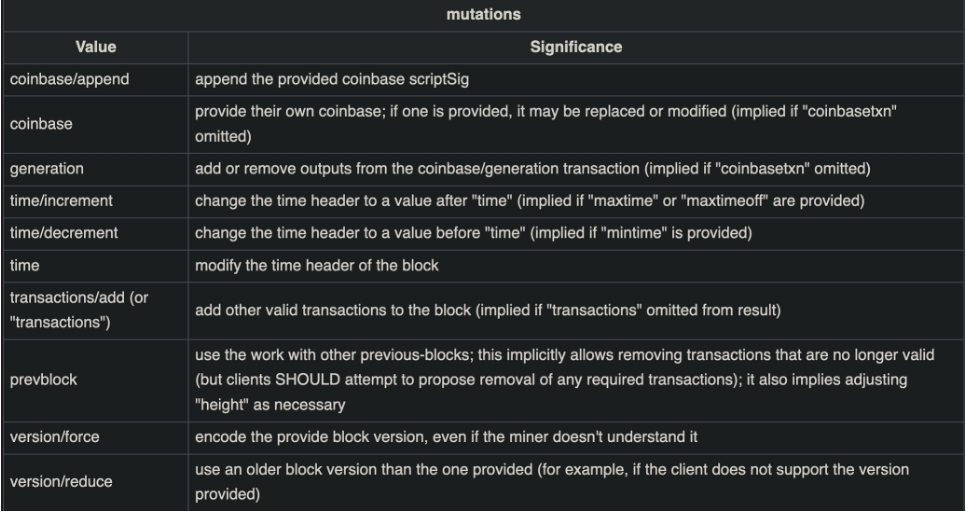
\includegraphics[width=15cm]{Figures/gbt/gbt3.png}
\caption{Mutations which can be asked from a miner, using GBT \cite{bitcoin0023Bitcoin}}
\label{fig:gbt3}
\end{figure}

\noindent At this point, pool server must return a JSON Object containing all the details needed to begin mining:
\begin{verbatim}
{"result": {
    "coinbasetxn": {
     "data": "010000000100000000000000000000000000000000000000000000
     00000000000000000000ffffffff1302955d0f00456c667697573005047dc66
     085fffffffff02fff1052a010000001976a9144ebeb1cd26d6227635828d60d
     3e0ed7d0da248fb88ac01000000000000001976a9147c866aee1fa2f3b3d5ef
     fad576df3dbf1f07475588ac00000000"
    },
    "previousblockhash": "000000004d424dec1c660a68456b8271d09628a80c
    c62583e5904f5894a2483c",
    "transactions": [],
    "expires": 120,
    "target": "00000000fffffffffffffffffffffffffffffffffffffffffffff
    fffffffffff",
    "longpollid": "some gibberish",
    "height": 23957,
    "version": 2,
    "curtime": 1346886758,
    "mutable": ["coinbase/append"],
    "bits": "ffff001d"
},"id": 0} 
\end{verbatim}

\begin{figure}[h!]
\centering
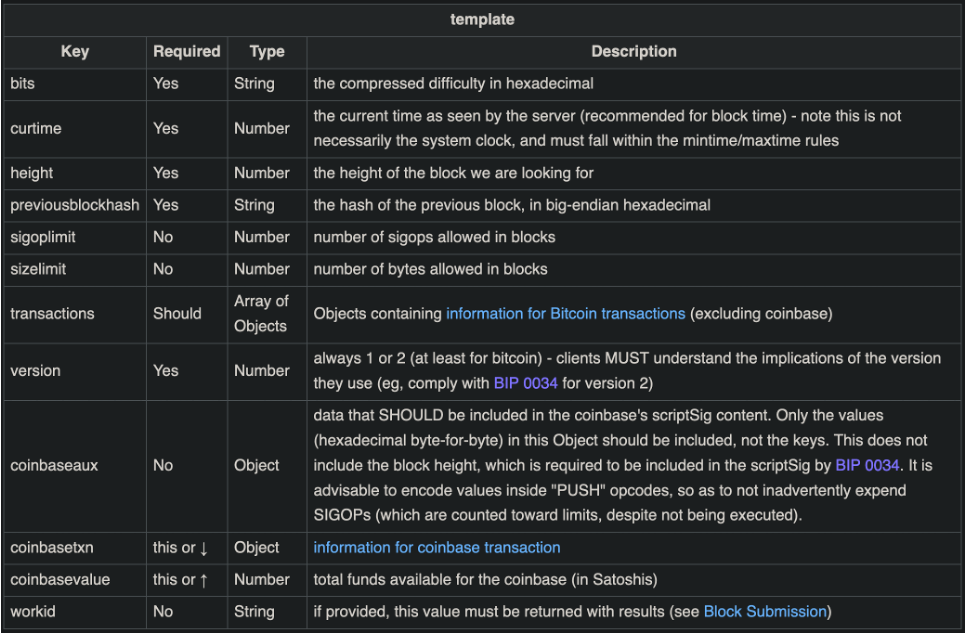
\includegraphics[width=15cm]{Figures/gbt/gbt4.png}
\caption{Description of the template fields sent by the mining pool, using GBT}
\label{fig:gbt4}
\end{figure}

\begin{figure}[h!]
\centering
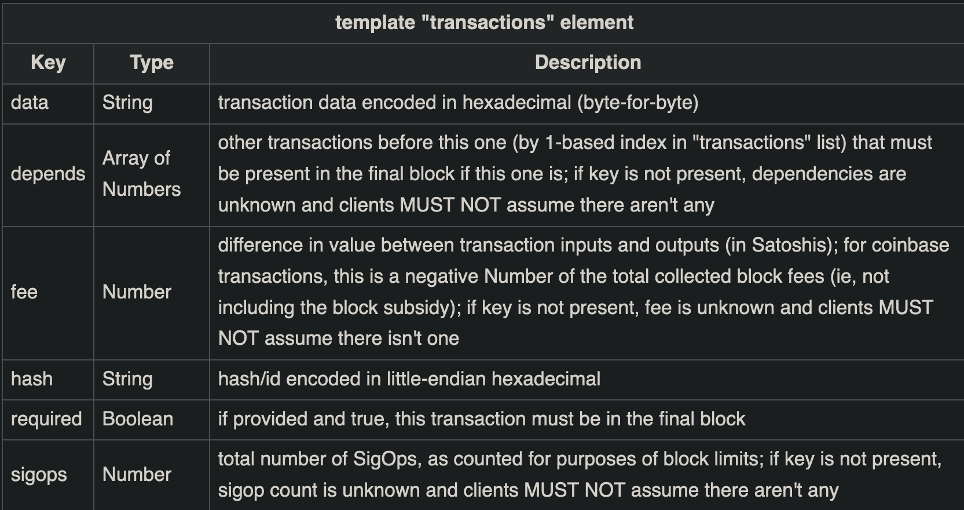
\includegraphics[width=15cm]{Figures/gbt/gbt5.png}
\caption{Transaction fields, present in the template sent by pool server, using GBT}
\label{fig:gbt5}
\end{figure}

\noindent In the template sent by pool server, the "mutable" key can be used to specify which modifications the miner is allowed to make, on that specific template.
In this specific case, the pool has agreed upon the miner request to edit the coinbase transaction, with can be used as an extranonce, to enlarge the nonce research space. This is specified by both miner template request and pool template response, in the "mutable" key field, as ["coinbase/append"] value.\\\\
So, as soon as the template is received, the miner needs to customize the coinbase transaction, with the only limitation about not exceeding the 100 bytes data limit. 
Coinbase data (which are the ones customizable) begins after 42 bytes, in the coinbase transaction, and the 42nd byte represents the data length. So, miner must insert the custom data right after the "original" data already present in the coinbase provided by pool server. At the end, it needs to change the 42nd byte, inserting the new data length. This is an example Python script which customizes the coinbase transaction data, inserting the 'my block' string:
\begin{lstlisting}[style=pythonStyle, numbers=none]
import binascii
coinbase = binascii.a2b_hex(template['coinbasetxn']['data'])
extradata = b'my block'
origLen = ord(coinbase[41:42])
newLen = origLen + len(extradata)
coinbase = coinbase[0:41] + chr(newLen).encode('ascii') + 
coinbase[42:42 + origLen] + extradata + coinbase[42+origLen:]
\end{lstlisting}
\medskip
Since the coinbase transaction data has been modified, the new merkle root needs to be re-built, before starting hashing on the new customized block header.
First, miner must put the modified coinbase transaction at the first place in the transactions list received from the pool server. At this point he needs to apply double SHA-256 to every transaction in the list; after that, he needs to redo the double SHA-256 to every couple of transactions (concatenated), as long as it remains just one single hash string, which is the final merkle root.
To do this, the following Python script can be used as an example:
\begin{lstlisting}[style=pythonStyle, numbers=none]
import hashlib
def dblsha(data):
 	return hashlib.sha256(hashlib.sha256(data).digest())
    .digest()

txnlist = [coinbase] + [binascii.a2b_hex(a['data']) 
for a in template['transactions']]
merklehashes = [dblsha(t) for t in txnlist]
while len(merklehashes) > 1:
	 if len(merklehashes) % 2:
	  	merklehashes.append(merklehashes[-1])
 	merklehashes = [dblsha(merklehashes[i] + merklehashes[i + 1])
  for i in range(0, len(merklehashes), 2)]
merkleroot = merklehashes[0]
\end{lstlisting}
Once the new merkle root has been computed, the new block header has to be assembled. To do this, miner can take the data already present in the template sent by pool server, substitute the merkle root with the one just computed, and start hashing on the customized block header.
\begin{lstlisting}[style=pythonStyle, numbers=none]
import struct
blkheader = struct.pack('<I', template['version']) + \
            binascii.a2b_hex(template['previousblockhash']) +
            merkleroot + \
            struct.pack('<I', template['curtime']) + \
            binascii.a2b_hex(template['bits']) + \
            b'NONC'
\end{lstlisting}
\medskip
Whenever the miner finds a share (or block) which is valid, he needs to send it immediately to the pool server, to be rewarded for it. To do this, a submitblock method is exploited, which requires just one parameter: the serialized block data.\\
To build a serialized block, miner needs to concatenate the block header, the number of transactions, and the transactions in the block (placed in the same order of the merkle tree used to compute the merkle root) \cite{bitcoinBlockChain}.
\begin{verbatim}
{"id": 0, 
    "method": "submitblock", 
    "params": ["020000003c48a294584f90e58325c60ca82896d071826b45680a6
    61cec4d424d00000000de6433d46c0c7f50d84a05aec77be0199176cdd47f77e3
    44b6f50c84380fddba66dc47501d00ffff0000010001010000000100000000000
    00000000000000000000000000000000000000000000000000000ffffffff1302
    955d0f00456c6967697573005047dc66085fffffffff02fff1052a01000000197
    6a9144ebeb1cd26d6227635828d60d3e0ed7d0da248fb88ac0100000000000000
    1976a9147c866aee1fa2f3b3d5effad576df3dbf1f07475588ac00000000"]
}
\end{verbatim}
\medskip
While the miner is hashing on the block header, changing nonce and time fields, he needs to be updated from the pool whenever a new block is found, to not wasting time and energy.
To achieve this, an optional long polling extension was designed into getblocktemplate protocol.
To use it, miner needs to explicitly indicate it in the template request message, like this:
\begin{verbatim}
{"id": 0, 
"method": "getblocktemplate", 
"params": [{
    "capabilities": ["coinbasetxn", "workid", "coinbase/append"],
    "longpollid": "some gibberish",
}]}
\end{verbatim}
In this way, as soon as a new block is found on the Bitcoin network, pool server can immediately notify the miner which is putting hash power into the pool.\\\\
In addition to the described "standard" behavior, getblocktemplate protocol permits many possible execution flows, depending on the mutations and pool extension used by the miner.
To investigate them more deeply, in the description of BIP23 there's a dedicated section for it: moreover, there are some interesting answers to basic questions and doubts which came out during the weeks which followed the publication of the protocol itself.
